\begin{frame}{Lineations and Boundaries}

\centering

\begin{tikzpicture}[x=1cm,y=0.85cm]

%=================================================
% LEFT COLUMN
%=================================================

% Crater

\fill (0.6,-0.5) circle (0.10);

\node[anchor=west,font=\small]
at (1.4,-0.5)
{Crater};

% Sharp boundary

\draw[line width=1pt]
(0,-1.6)--(1.2,-1.6);

\node[anchor=west,font=\small]
at (1.4,-1.6)
{Sharp boundary};

% Broad flow-parallel

\draw[
-{Triangle[length=8pt,width=9pt]},
line width=1.4pt
]
(0,-2.7)--(1.2,-2.7);

\node[anchor=west,font=\small]
at (1.4,-2.7)
{Broad flow-parallel lineation};

% Fine flow-parallel

\draw[
-{Triangle[length=7pt,width=7pt,open]},
line width=0.9pt
]
(0,-3.8)--(1.2,-3.8);

\node[anchor=west,font=\small]
at (1.4,-3.8)
{Fine flow-parallel lineation};

% Broad flow-transverse

\draw[red,line width=1.1pt]
(0,-4.9)--(1.2,-4.9);

\foreach \x in {0.25,0.60,0.95}
{
\draw[red,line width=1.1pt]
(\x,-5.1)--(\x,-4.7);
}

\node[anchor=west,font=\small]
at (1.4,-4.9)
{Broad flow-transverse lineation};

% Fine flow-transverse

\draw[red,line width=0.8pt]
(0,-6.0)--(1.2,-6.0);

\foreach \x in {0.25,0.60,0.95}
{
\draw[red,line width=0.8pt]
(\x,-6.15)--(\x,-5.85);
}

\node[anchor=west,font=\small]
at (1.4,-6.0)
{Fine flow-transverse lineation};

%=================================================
% RIGHT COLUMN
%=================================================

% Scarp top

\draw[line width=1pt]
(7.0,-1.0)--(8.3,-1.0);

\foreach \x in {7.3,7.8,8.2}
{
\draw[line width=0.8pt]
(\x,-1.0)--(\x,-1.3);
}

\node[anchor=west,font=\small]
at (8.7,-1.0)
{Scarp top};

% Scarp base

\draw[line width=1pt]
(7.0,-2.2)--(8.3,-2.2);

\fill
(7.65,-2.0)--(7.50,-2.2)--(7.80,-2.2)--cycle;

\node[anchor=west,font=\small]
at (8.7,-2.2)
{Scarp base};

% Ridge crest

\draw[line width=1pt]
(7.3,-3.6)--(8.1,-3.6);

\draw[line width=1pt]
(7.3,-4.0)--(8.1,-3.2);

\draw[line width=1pt]
(7.3,-3.2)--(8.1,-4.0);

\node[anchor=west,font=\small]
at (8.7,-3.6)
{Ridge crest};

% Trough

\draw[line width=1pt]
(7.1,-5.1)--(8.2,-5.1);

\fill
(7.65,-4.8)--(7.45,-5.1)--(7.85,-5.1)--cycle;

\fill
(7.65,-5.4)--(7.45,-5.1)--(7.85,-5.1)--cycle;

\node[anchor=west,font=\small]
at (8.7,-5.1)
{Trough};

% Rib

\draw[green!70!black,line width=1.3pt]
(7.0,-6.3)--(8.3,-6.3);

\node[anchor=west,font=\small]
at (8.7,-6.3)
{Rib};

\end{tikzpicture}

\end{frame}

%%%%%%%%

\begin{frame}{Lineations and Boundaries: Gradational / Degraded}

\centering

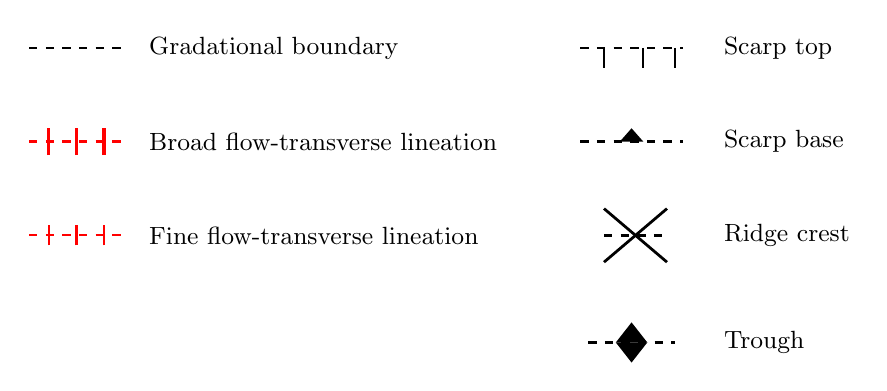
\begin{tikzpicture}[x=1cm,y=0.85cm]

%=================================================
% LEFT COLUMN
%=================================================

% Gradational boundary

\draw[dashed,line width=1pt]
(0,-1.0)--(1.2,-1.0);

\node[anchor=west,font=\small]
at (1.4,-1.0)
{Gradational boundary};

%  broad flow-transverse

\draw[red,dashed,line width=1.1pt]
(0,-2.4)--(1.2,-2.4);

\foreach \x in {0.25,0.60,0.95}
{
\draw[red,line width=1.1pt]
(\x,-2.6)--(\x,-2.2);
}

\node[anchor=west,font=\small]
at (1.4,-2.4)
{ Broad flow-transverse lineation};

%  fine flow-transverse

\draw[red,dashed,line width=0.8pt]
(0,-3.8)--(1.2,-3.8);

\foreach \x in {0.25,0.60,0.95}
{
\draw[red,line width=0.8pt]
(\x,-3.95)--(\x,-3.65);
}

\node[anchor=west,font=\small]
at (1.4,-3.8)
{ Fine flow-transverse lineation};

%=================================================
% RIGHT COLUMN
%=================================================

%  Scarp top

\draw[dashed,line width=1pt]
(7.0,-1.0)--(8.3,-1.0);

\foreach \x in {7.3,7.8,8.2}
{
\draw[line width=0.8pt]
(\x,-1.0)--(\x,-1.3);
}

\node[anchor=west,font=\small]
at (8.7,-1.0)
{ Scarp top};

%  Scarp base

\draw[dashed,line width=1pt]
(7.0,-2.4)--(8.3,-2.4);

\fill
(7.65,-2.2)--(7.50,-2.4)--(7.80,-2.4)--cycle;

\node[anchor=west,font=\small]
at (8.7,-2.4)
{ Scarp base};


% Ridge crest
\draw[dashed,line width=1pt]
(7.3,-3.8)--(8.1,-3.8);
\draw[line width=1pt]
(7.3,-4.2)--(8.1,-3.4);
\draw[line width=1pt]
(7.3,-3.4)--(8.1,-4.2);
\node[anchor=west,font=\small]
at (8.7,-3.8)
{ Ridge crest};

%  Trough

\draw[dashed,line width=1pt]
(7.1,-5.4)--(8.2,-5.4);

\fill
(7.65,-5.1)--(7.45,-5.4)--(7.85,-5.4)--cycle;

\fill
(7.65,-5.7)--(7.45,-5.4)--(7.85,-5.4)--cycle;

\node[anchor=west,font=\small]
at (8.7,-5.4)
{ Trough};

\end{tikzpicture}

\end{frame}